\documentclass{article}
\usepackage[utf8]{inputenc}
\usepackage[T1]{fontenc}
\usepackage[french]{babel}
\usepackage{graphicx}
\usepackage{multimedia}
\usepackage[top=3cm, bottom=4cm, left=3cm, right=3cm, a4paper]{geometry}
\usepackage{lipsum}
\usepackage{caption}
\usepackage{fancyhdr}
\usepackage{tabto}
\usepackage{xcolor}
\usepackage{array}
\usepackage{enumitem}
\usepackage{eurosym}
\usepackage{xcolor}
\usepackage{blindtext}
\definecolor{back}{rgb}{0.15, 0.15, 0.15}
\usepackage[T1]{fontenc}
\usepackage[utf8]{inputenc}
\usepackage{geometry}
\usepackage{multirow}
\usepackage{mathtools}
\usepackage{amsmath}
\usepackage{systeme}

\usepackage{listings}
\definecolor{mygreen}{rgb}{0,0.6,0}
\definecolor{mygray}{rgb}{0.5,0.5,0.5}
\definecolor{mymauve}{rgb}{0.58,0,0.82}
\definecolor{whiteback}{rgb}{0.95, 0.95, 0.95}

\lstset{
language=c,
basicstyle=\footnotesize\ttfamily,
numbers=left,
numberstyle=\tiny,
numbersep=5pt,
tabsize=2,
extendedchars=true,
breaklines=true,
frame=b,
stringstyle=\color{mygreen}\ttfamily,
showspaces=false,
showtabs=false,
xleftmargin=0pt,
xrightmargin=0pt,
columns=fullflexible,
framexleftmargin=15pt,
framexrightmargin=0pt,
framexbottommargin=10pt,
framextopmargin=15pt,
commentstyle=\color{mygreen},
morecomment=[l]{//},
morecomment=[s]{/*}{*/},
showstringspaces=false,
morekeywords={ abstract, event, new, struct,
as, explicit, null, switch,
base, extern, object, this,
bool, false, operator, throw,
break, finally, out, true,
byte, fixed, override, try,
case, float, params, typeof,
catch, for, private, uint,
char, foreach, protected, ulong,
checked, goto, public, unchecked,
class, if, readonly, unsafe,
const, implicit, ref, ushort,
continue, in, return, using,
decimal, int, sbyte, virtual,
default, interface, sealed, volatile,
delegate, internal, short, void,
do, is, sizeof, while,
double, lock, stackalloc,
else, long, static,
enum, namespace, string},
keywordstyle=\color{blue},
identifierstyle=\color{back},
backgroundcolor=\color{whiteback},
}

\setcounter{page}{1}
\usepackage{fancyhdr}
\pagestyle{fancy}
\renewcommand{\headrule}{{\color{gray}\vskip-\footruleskip\vskip-\footrulewidth \hrule width\headwidth height\footrulewidth\vskip\footruleskip}}
\renewcommand{\footrule}{{\color{gray}\vskip-\footruleskip\vskip-\footrulewidth \hrule width\headwidth height\footrulewidth\vskip\footruleskip}}
\renewcommand{\footrulewidth}{0.5pt}

\rhead{}
\lhead{}


\usepackage{tocloft}


\begin{document}

    \headsep = 12pt
    \vspace*{\stretch{1}}
		\begin{center}
			\begin{LARGE}
				\textbf{Rapport de soutenance}
				\paragraph{}Charles\hspace{0.7cm}Quentin\hspace{0.7cm}Maxime\hspace{0.7cm}Nathan
			\end{LARGE}
		\end{center}
		\vspace{1.5cm}
		\begin{center}
			
\includegraphics[scale=0.3]{LogoBitarrays.png}
		\end{center}
		\begin{center}
			\par Par Bitarrays | Projet "Lambda"
		\end{center}
		\vspace*{\stretch{1}}
	
	\newpage
    \pagestyle{fancy}
    \fancyhf{}
    \lhead{Rapport de soutenance\vspace{0.25cm}}
    \rhead{Table des matières}
    \cfoot{\thepage}
    \chead{
\includegraphics[scale=0.05]{LogoBitarrays.png}}
    \tableofcontents
    
\newpage
\rhead{\textit{Prologue}\vspace{0.25cm}}
\cfoot{\thepage}
\chead{
\includegraphics[scale=0.05]{LogoBitarrays.png}}
\vspace*{5cm}
\begin{huge}
\hspace{-0.9cm}
\textbf{\emph{Prologue}}
\end{huge}
\vspace*{1cm}
\vspace{0.4cm}
	\paragraph{}
    Voici le premier rapport de soutenance pour notre projet d'OCR à réaliser en groupe de 4 étudiants. L'objectif est de répondre pleinement au cahier des charges imposé par l'école et obtenir un résultat satisfaisant dans la reconnaissance des caractères.
	
	\paragraph{}
    Nous n'avons pas eu de phase de réflexion sur le projet pour cette année et sommes directement entrés dans le vif du sujet et la réalisation des tâches obligatoires pour respecter scrupuleusement les deadlines du projet et ne pas prendre de retard. Il nous fallait nous familiariser avec le langage C et comprendre les attentes du projet.
	
	\paragraph{}
    Nous allons apprendre à communiquer et à s'adapter aux différents caractères des membres de notre groupe. Nous avons, par expérience, déjà compris qu'un projet de groupe est un réel défi au niveau humain mais ce projet s'annonce encore plus complexe.
    Nous sommes tous très motivés par la création de l'OCR.
	
	\paragraph{}
    Ce fut un gros investissement pour nous 4 durant ce premier mois pour proposer une segmentation des caractères convenable ainsi que le début de la réalisation de plusieurs éléments qui rendront notre OCR fonctionnel pour la date de la deuxième soutenance.

	\paragraph{}
    Nous allons présenter ici nos réalisation ainsi que nos problèmes rencontrés jusqu'à aujourd'hui.

\newpage
\lhead{Rapport de soutenance\vspace{0.25cm}}
\rhead{\textit{Présentation}\vspace{0.25cm}}
\vspace*{2cm}
\section{Présentations}
\subsection{Les membres}
\subsubsection{Quentin "Scout" FISCH}
\paragraph{}J'ai vraiment découvert ma passion pour l'informatique par le biais de TP effectués en Sciences de L'ingénieur en Première et Terminale. J'ai donc décider d'étudier car je suis très intéressé en ce qui concerne la robotique et le développement de technologies dans les systèmes embarqués. Ce projet sera pour moi le premier en langage C et m'apprendra comment gérer un tel projet en respectant des deadlines et diverses contraintes. Je suis ainsi très motivé à sortir le meilleur projet possible et développer mes compétences en informatique.

\subsubsection{Maxime "Maxmad" MADRAU}
\paragraph{}Passionné d'informatique depuis toujours, j'ai commencé a développer des programmes simples très tôt dans mon enfance. J'ai par la suite appris des langages comme le Python, le Lua, le Javascript, le Swift, et les langages web comme le HTML et le CSS. Mes domaines de prédilection sont les applications mobiles, les bases de données et le client/serveur.

\subsubsection{Charles "Draze" SIMON-MEUNIER}
\paragraph{}Passionné d'informatique depuis mes années du collège ou j'ai commencé à développer des serveurs sur Minecraft, EPITA est pour moi une révélation. Une école avec une formation permettant d'atteindre le statut d'ingénieur ainsi que des compétences en informatique plus que confortables est pour moi le cursus idéal. J'ai appris par moi même certains langages comme le HTML/CSS, Java et aujourd'hui je me perfectionne et corrige mes défauts grâce à l'école. Ce projet devrait m'apporter à titre personnel beaucoup d'expérience, autant au niveau humain que dans les compétences informatiques.

\subsubsection{Nathan "Goruza" AVÉ}
\paragraph{}Après une première année de sup ou j’ai pu vivre ma première expérience de travail de groupe à EPITA, je poursuis l’aventure avec plus d’expérience dans les projets de ce type et aussi un groupe différent. Pour moi, l’OCR est une seconde expérience de travail où je vais devoir apprendre à maitriser des notions par moi-même et non pas lors des cours. Cela s’inscrit dans la continuité de mon stage réalisé cet été par l’apprentissage d’un nouveau langage et la similarité de mes collègues pour ce projet ayant fait ce stage avec Quentin et Charles. Préparez-vous ce projet sera légendaire !


\newpage

\vspace*{\stretch{1}}

\subsection{Le groupe}

\paragraph{}Nous avons créé notre groupe en reprenant les membres avec qui nous avions travaillé l'année dernière car l'entente était très bonne tout comme l'efficacité au sein du groupe. De plus, nous avons déjà quelques projets de groupe à notre actif ce qui permet de connaître les points forts et faibles de chacun. Malheureusement nous n'étions que 3 et il fallait trouver un dernier membre pour former un groupe de 4 personnes. Nathan était le bon candidat car nous nous connaissons bien et le travail pourrait alors être efficace.

\paragraph{}Comme nous avons l'habitude de travailler ensemble, nous savons comment chacun fonctionne et comment chacun réalise ses tâches. Maxime est plus solitaire mais très acharné et réussi donc toujours à réaliser ce qu'il doit faire, Nathan sait innover et trouver les idées pour apporter des améliorations sur des réalisations tandis que Quentin et Charles arrivent à travailler efficacement en binôme plutôt que seuls.

\paragraph{}Avec ses données, chacun a pu trouver dans ce projet sa place et fournir un travail qui permet de répondre aux attentes de cette première soutenance. Tout ce que nous avons développé n'est pas parfait mais les idées sont là et ne peuvent qu'être améliorées par la suite.

\paragraph{}Ainsi l'entente au sein du groupe est très bonne et devrait permettre de continuer dans ce projet motivant pour révéler le meilleur de chacun et pouvoir réaliser des bonus et rendre notre projet utilisable par la suite.

\paragraph{}Notre groupe de projet pour le même nom que l'année dernière (Bitarrays) car nous avons continué de le faire vivre après la fin du projet de S2. Nous avons décidé de donner le nom Lambda à notre projet de cette année.

\vspace*{0.5cm}
\begin{center}
	
\includegraphics[scale=0.4]{work}
\end{center}

\vspace*{\stretch{1}}

\newpage

\rhead{\textit{Pré-traitement}\vspace{0.25cm}}
\section{Traitement de l'image (pré-traitement)}

\subsection{Ce que nous devions faire}

\paragraph{}Pour traiter les images de la meilleure des façons, il fallait penser à réaliser un pré traitement sur ces dernières pour que notre segmentation soit la meilleure possible. Il fallait réaliser un niveau de gris, une binarisation et appliquer des filtres permettant de réduire le bruit sur l'image. Toute cette partie est réalisée dans le fichier filters.c, contenu dans \textbf{"/src/ImageTreatment"}

\subsection{Le niveau de gris}

\paragraph{}Rien de compliqué pour réaliser cette fonction, il suffit de parcourir entièrement l'image et d'appliquer pour chacun des pixels une nouvelle valeur utilisant les valeurs de rouge, vert et bleu de chaque pixel. Les coefficients appliqués aux valeurs rouge, vert et bleu sont respectivement 0.3, 0.59, 0.11. Cela permet de créer un nouveau pixel avec cette nouvelle valeur pour sa valeur rouge, vert et bleu (pour obtenir un niveau de gris).

\paragraph{}Pour utiliser cette fonctionnalité dans notre programme, il suffit d'exécuter
\begin{lstlisting}
./Lambda grayscale "image_path" "destination_path"
\end{lstlisting}

\paragraph{}Et voici le résultat obtenu une fois le programme exécuté
\begin{center}
	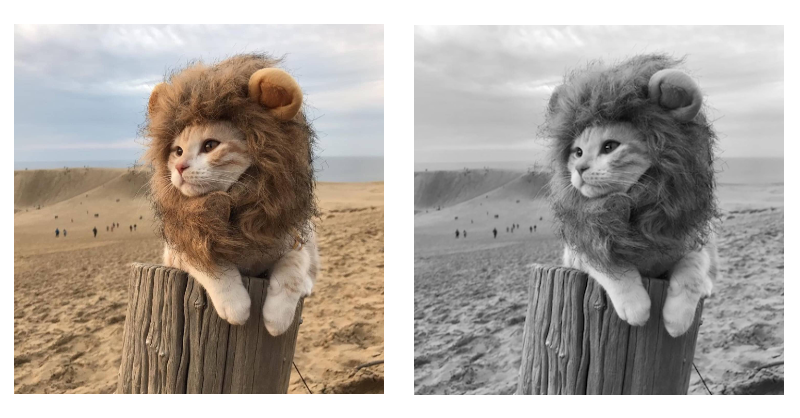
\includegraphics[scale=0.45]{a}
\end{center}


\subsection{Binarisation}

\paragraph{}Pour binariser l'image (c'est à dire ne laisser que des pixels blancs ou noirs), nous avons appliqué une condition simple sur chacun des pixels qui composent l'image. Nous faisons la moyenne des valeurs rouge, vert et bleu et vérifions si cette dernière est supérieure ou non à 127. Si elle est supérieure, nous mettons un pixel blanc et un noir sinon. Il n'existe pas de commande pour appliquer ce filtre dans notre exécutable.xel blanc et un noir sinon. Il n'existe pas de commande pour appliquer ce filtre dans notre exécutable.
\paragraph{} Ce n'est pas ici la fonction la plus compliquée de notre code mais ce sont des éléments essentiels pour la suite.

\newpage

\subsection{Augmentation des contrastes}

\paragraph{}Sur certaines images, les contrastes ne sont pas assez prononcés et il faut alors les augmenter. Pour cela, nous avons créé une fonction utilisant un histogramme normalisé de tous les pixels d'une image en niveaux de gris. L'histogramme est représenté par une liste de taille 256.

\paragraph{}Comme l'image traitée est en niveau de gris, nous construisons l'histogramme en parcourant chaque pixel et en ajoutant la valeur rouge du pixel par exemple (comme les valeurs de rouge, bleu et vert sont les mêmes).

\paragraph{}Ensuite, l'objectif est de trouver une nouvelle valeur pour chaque pixel de l'image. Pour cela, nous repassons à nouveau dans chaque pixel et utilisons la formule:\newline
\begin{center}
	$\sum_{n=0}^{k}\frac{255}{nbPixels}*histogram[n]$
\end{center}

\paragraph{}qui correspond à la somme du nombre de pixels de l'image dont la valeur est inférieure ou égale au pixel traité. Nous multiplions ensuite cette donnée par $\frac{255}{nbPixels}$ pour normaliser et obtenir la nouvelle valeur de gris du pixel.


\subsection{Réduction des bruits}

\paragraph{}Nous n'appliquons ce filtre que sur des images en niveaux de gris.

\paragraph{}Pour réduire les bruits sur l'image, nous suivons un algorithme qui s'applique sur chaque pixel. Nous faisons la somme des valeurs des pixels voisins (les 8 pixels qui entourent le pixel actuel s'ils existent). La valeur du nouveau pixel est la moyenne des valeurs des pixels voisins.

\paragraph{}Voici la fonction qui est utilisée dans notre code

\begin{lstlisting}
	// Foreach pixels
    for (int i = 0; i < img->w; i++)
    {
        for (int j = 0; j < img->h; j++)
        {
            // Sum of each neighbors pixels
            Uint32 sum = 0;
            short count = 0;
            for (int k = -1; k < 2; k++)
            {
                for (int l = -1; l < 2; l++)
                {
                    if (i + k > -1 && 
                        i + k < img->w && 
                        j + l > - 1 && 
                        j + l < img->h) 
                    {
                        pixel = getpixel(img, i + k, j + l);
                        SDL_GetRGB(pixel, img->format, &r, &g, &b);
                        sum += r;
                        count += 1;
                    }
                }
            }
            // Average of pixels values to get the new current pixel value
            sum /= count;
            pixel = SDL_MapRGB(img->format, sum, sum, sum);
            putpixel(imgCopy, i, j, pixel);
        }
    }
\end{lstlisting}

\section{Rotation de l'image}
\subsection{Rotation manuelle}
\paragraph{}
Nous avons implémenté une rotation manuelle de l'image, c'est-à-dire qu'une rotation de l'image est effectuée pour un angle donné en paramètre. Ainsi, nous pourrions créer un input sur l'interface afin que l'utilisateur puisse dire lui-même de combien de degrés l'image doit être tournée pour être droite lors de la détection du texte. Cependant, nous avons choisi de ne pas implémenter ce fonctionnement directement, mais de créer une fonction qui détecte automatiquement l'angle de l'image. Nous reviendrons sur ce choix et cette fonction dans la partie suivante.

\paragraph{}
Pour ce qui est de la fonction qui retourne une image de façon manuelle, voici comment celle-ci fonctionne: \\

\begin{lstlisting}

	SDL_Surface *rotation(SDL_Surface *img, double teta, int x0, int y0) {
        SDL_Surface *imgCopy = SDL_CreateRGBSurface(0, img->w, img->h, 32, 0, 0, 0, 0);
        
        // Full white image
        pixel = SDL_MapRGB(img->format, 255, 255, 255);
        for (int i = 0; i < img->w; i++) {
            for (int j = 0; j < img->h; j++) {
                putpixel(imgCopy, i, j, pixel);
            }
        }
        
        teta = toradians(teta);

        for (int x = 0; x < img->w; x++) {
            for (int y = 0; y < img->h; y++) {
                int x2 = round(cos(teta) * (double)(x - x0) + sin(teta) * (double)(y - y0));
                int y2 = round(cos(teta) * (double)(y - y0) - sin(teta) * (double)(x - x0));
                
                x2 += x0;
                y2 += y0;
                if (x2 > -1 && x2 < img->w && y2 > -1 && y2 < img->h ) {
                    putpixel(imgCopy, x2, y2, getpixel(img, x, y));
                }
            }
        }
        return imgCopy;
    }
\end{lstlisting}

\paragraph{}
Cette fonction est plutôt simple dans sa manière de fonctionner. Tout d'abord, on créer une nouvelle image toute blanche de la même taille que l'image passée en paramètre. C'est le but de la première boucle de la fonction. Ensuite, on redéfini l'angle $\theta$ donné en paramètre en radian, ce qui permet ensuite d'utiliser les fonctions \textit{sin()} et \textit{cos()} de la librairie \textit{Math.h}. 
\par Pour ce qui est de la rotation en elle-même de l'image, on parcours tous les pixels de l'image grâce aux deux boucles \textit{for} imbriquées. On calcule les nouvelles coordonnées du pixel grâce à la formule suivante: \\
\[
\systeme*{x_2 = cos(\theta)*(x - x_0) + sin(\theta)*(y - y_0), y_2 = cos(\theta)*(y - y_0) + sin(\theta)*(x - x_0)}
\] \\
Après avoir calculé les nouvelles coordonnées, on ajoute $x_0$ à $x_2$ et $y_0$ à $y_2$ pour centrer la rotation. Finalement, il suffit d'ajouter le pixel sur lequel on est placé aux nouvelles coordonnées sur la nouvelle image. Le résultat est le bon, mais on obtient des pixels manquant sur l'image:

$Image_pixels_manquants$

\paragraph{}
Nous avons essayé plusieurs algorithmes pour corriger ce problème, mais nous n'avons pas eu de résultats concluant qui supprimaient totalement ce problème. C'est le défaut d'effectuer une rotation de l'image avant de traiter le texte.

\subsection{Rotation automatique}

\newpage
\rhead{\textit{Segmentation de l'image}\vspace{0.25cm}}
\section{Segmentation de l'image}
\subsection{Introduction}
    \paragraph{}
    Ce premier mois de projet nous a permis de commencer à implémenter des fonctionnalités primordiales pour la réalisation de notre projet final. En effet nous avons réalisé la segmentation des caractères, à reconnaître par la suite. \\
    Ce processus est complexe et crucial pour pouvoir fournir au programme de reconnaissance des caractères bien découpés et formalisés comme le dataset utilisé pour l'entraîner.
    
\subsection{Segmentation de caractères}
    \paragraph{}
    Comme dit précédemment, la segmentation du texte initial en caractères reconnaissables par le programme est une des parties sur laquelle nous nous sommes le plus penché durant ce premier mois.
    
    \subsubsection{Découpage des colonnes}
    \paragraph{}
    Si la détection des caractères est primordiale, elle n'est que le point final du chaîne d'opérations sur l'image initiale. La première étape du processus de segmentation est le découpage des colonnes. Par exemple, l'image présentée ci-dessous comporte deux colonnes, qu'il faut séparer pour pouvoir continuer le processus de segmentation. \\
    
    \begin{center}
    	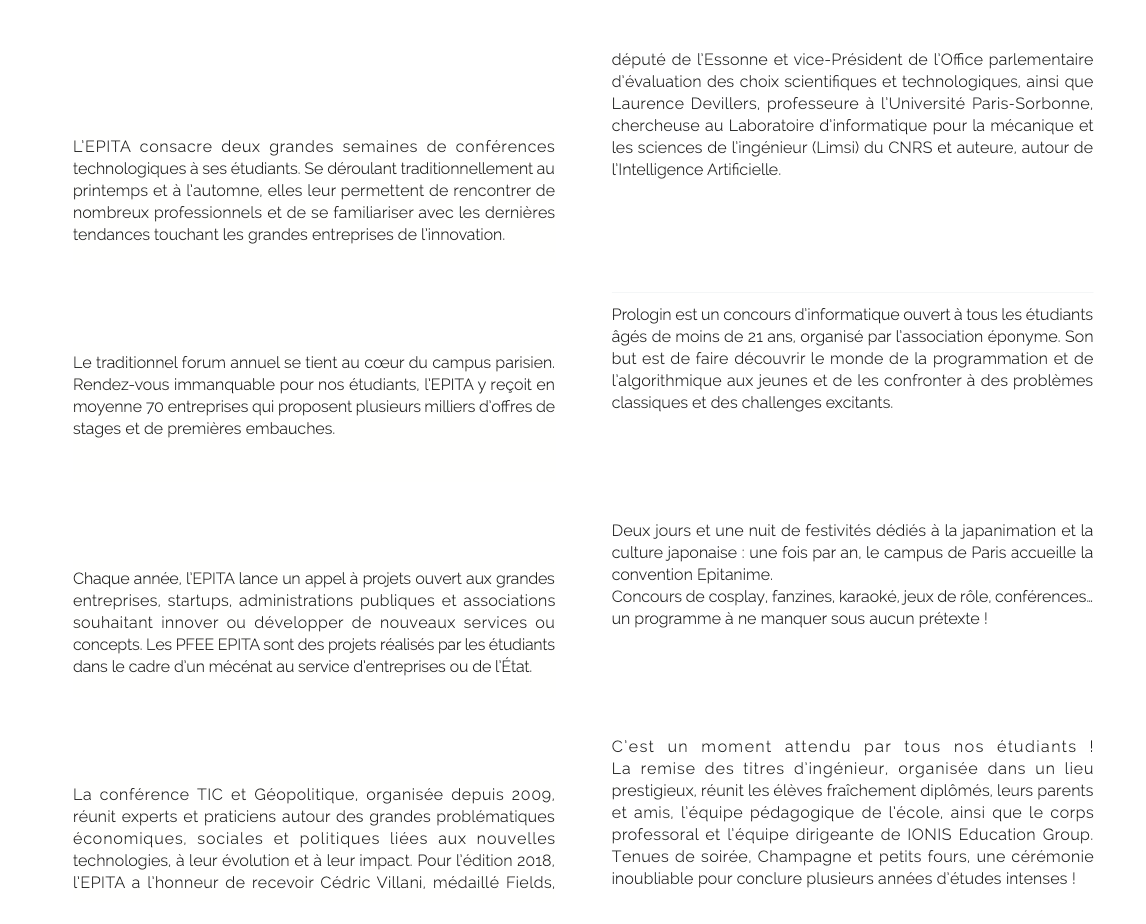
\includegraphics[scale=0.3]{paragraph}
    \end{center}
    
    \paragraph{}
    La détection des colonnes est un processus assez simple, qui tient compte de la "logique" d'organisation d'un texte. En effet, en tant qu'humains, nous distinguons deux colonnes comme des "colonnes" et non une suite de mots par l'espace situé entre les deux blocs qui est anormalement grand par rapport aux espaces présents entre les mots du texte.
    \par
    Ainsi, nous avons implémenté la même logique pour la segmentation, qui détecte un espace rempli de pixels blancs anormalement grand entre deux parties ne contenant pas uniquement des pixels blancs. Voici un aperçu du code implémenté:
    
    \begin{lstlisting}
    
    unsigned char fullWhite = 1;
    unsigned char firstCut = 1;
    int endText = -1; //Gets the first pixel (width wise) with full white width
    int beginingText = -1; //Gets the first pixel without full white height after several full white 
    lastLineWidth = 0.03 * img -> w;
    
		for (int i = 0; i < img -> w; i++) 
    {
        // Returns whether img's height is full of white pixels or not
        fullWhite = fullWhite(img, i);

        if (!fullWhite && firstCut)
        {   
            // Begins column cut
            beginingText = i;
            if (endText == -1 || lastLineWidth <= abs(endText - beginingText)){
                //Draw line to separate column
                for (int k = 0; k < img -> h; k++)
                {
                    pixel = SDL_MapRGB(img_copy -> format, 0, 255, 0);
                    putpixel(img_copy, beginingText, k, pixel);
                }   
            }
            firstCut = 0;
        }
        
        if(fullWhite && !firstCut) {
        
            // Ends column cut
            endText = i-1;
            int ii = i;
            do
            {
                fullWhite = fullWhite(img, ii);
                ii++;
            } while (fullWhite);
            
            if (ii - endText >= lastLineWidth || ii >= img -> w) {
                // Space is too big, draw line to separate
                for (int k = 0; k < img -> h; k++)
                {
                    pixel = SDL_MapRGB(img_copy -> format, 0, 255, 0);
                    putpixel(img_copy, i, k, pixel);
                }
            }
            firstCut = 1;
        }
    }	
	\end{lstlisting}
	\vspace*{0.5cm}
	\par
	Le principe est le suivant: on possède une variable \textit{fullWhite} qui indique si, pour un pixel donné (sur la largeur), tous les pixels sur la hauteur de l'image sont blancs. Cette variable est très importante, car combinée à \textit{firstCut}, on peut savoir si la partie de l'image où l'on se situe est du texte ou non. \textit{firstCut} permet de savoir si nous sommes en train de chercher le début d'une colonne (1 dans ce cas), ou si le début la colonne est déjà repéré et qu'on cherche donc la fin.
	
	\paragraph{}
	Ainsi le code devient plus compréhensible. En parcourant toute la largeur de l'image, on regarde à chaque fois si toute la hauteur de l'image est blanche. 
	\par
	Si c'est n'est pas cas et que nous cherchons le début d'une colonne, alors nous l'avons trouvé et pouvons dessiner une ligne verticale pour marquer le début de la colonne.
	\par
	Si cependant nous ne cherchons plus le début mais la fin d'une colonne et qu'on se trouve sur un pixel dont la hauteur de l'image est toute blanche, alors nous évaluons les possibilités que ce soit la fin de la colonne. On note \textit{endText} comme l'indice final temporaire du texte. On continue d'avancer dans la largeur de l'image jusqu'au prochain pixel qui n'est pas \textit{fullWhite}. Enfin, la distance entre ce nouveau pixel et \textit{endText} est comparée à une constant représentant 3\% de la largeur de l'image. Si l'écart est supérieur à cette constante, on considère l'espace comme trop grand pour être un espace entre deux mots et on coupe la fin de la colonne au niveau de \textit{endText}. \\
	
	\paragraph{}
	Le résultat de ce programme sur la photo précédente donne l'image ci-dessous, comportant en vert les lignes tracées par la programme pour délimiter les colonnes, qui peuvent maintenant être coupées: \\
	
	\begin{center}
		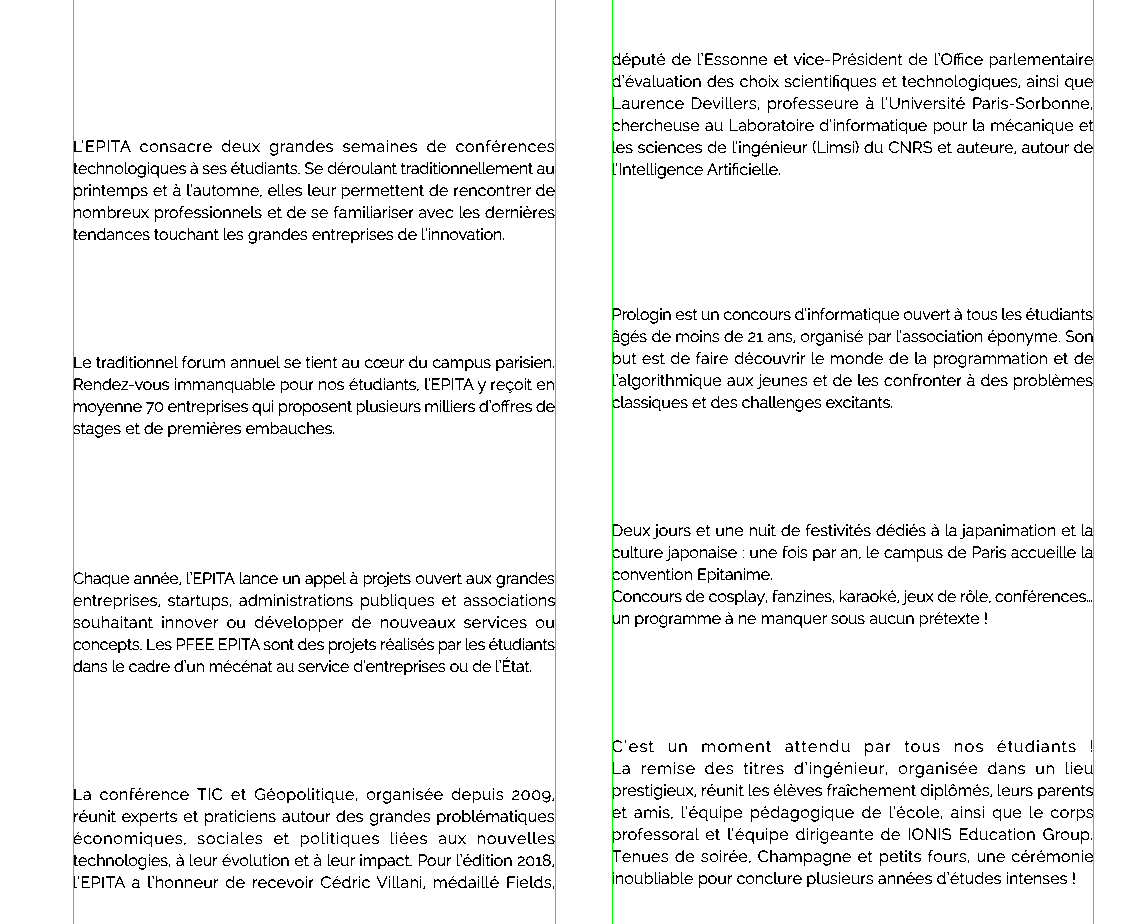
\includegraphics[scale=0.3]{columns}
	\end{center}
	
	\paragraph{}
	Comme vous pouvez le voir, quatre lignes sont créées: la première correspond au début de la première question, la deuxième à la fin de cette même colonne. Les deux autres représentent respectivement le début et la fin de la deuxième colonne. Bien entendu, ici, les colonnes sont juste découpées par des lignes, mais il faudrait les séparer en deux images différentes, ce qui est fait par une autre fonction de notre programme.
	
	\subsubsection{Découpage des paragraphes}
	\paragraph{}
	Cette partie est la suite logique du découpage des colonnes. En effet, en regardant l'image précédemment affichée, chaque colonne contient plusieurs paragraphes nettement distinguables. Ainsi, un programme similaire est utilisé sur chaque colonne trouvée pour découper les différents paragraphes afin qu'ils soient traités plus tard.
	\par
	Ici, le changement est principalement basé sur le fait de regarder si la largeur de l'image est complètement blanche, contrairement à la hauteur pour les colonnes. De plus, on détermine ici si un paragraphe se termine en fonction de la "hauteur" de la dernière ligne/du dernier paragraphe trouvé. Voici le nouveau code pour ce type de segmentation: \\
	
	\begin{lstlisting}
    unsigned char fullWhite = 1;
    unsigned char firstCut = 1;
    int endText = -1; //Gets the first pixel (height wise) with full white width
    int beginingText = -1; //Gets the first pixel without full white width after several full white 
    int lastLineHeight = -1; //Stores the number of pixels from the last text line
    
		for (int i = 0; i < img -> w; i++) 
    {
        // Returns whether img's height is full of white pixels or not
        fullWhite = fullWhite(img, i);

        if (!fullWhite && firstCut)
        {   
            // Begins column cut
            beginingText = i;
            if (endText == -1 || (lastLineHeight <= abs(endText - beginingText)){
                for (int k = 0; k < img -> w; k++)
                {
                    pixel = SDL_MapRGB(img_copy -> format, 0, 255, 0);
                    putpixel(img_copy, k, beginingText, pixel);
                }   
            }
            firstCut = 0;
        }
        
        if(fullWhite && !firstCut) {
        
            // Ends column cut
            endText = i-1;
            lastLineHeight = endText - beginingText;
            int ii = i;
            do
            {
                fullWhite = fullWhite(img, ii);
                ii++;
            } while (fullWhite);
            
            if (ii - endText >= lastLineWidth || ii >= img -> h) {
                // Space is too big, draw line to separate
                for (int k = 0; k < img -> w; k++)
                {
                    pixel = SDL_MapRGB(img_copy -> format, 0, 255, 0);
                    putpixel(img_copy, k, i, pixel);
                }
            }
            firstCut = 1;
        }
    }	
	\end{lstlisting}
	
	\paragraph{}
	Le résultat de ce nouveau programme, combiné à une fonction qui retire les lignes vertes créées, découpe et stocke les paragraphes dans de nouvelles images donne le résultat suivant: 
	
	\begin{center}
		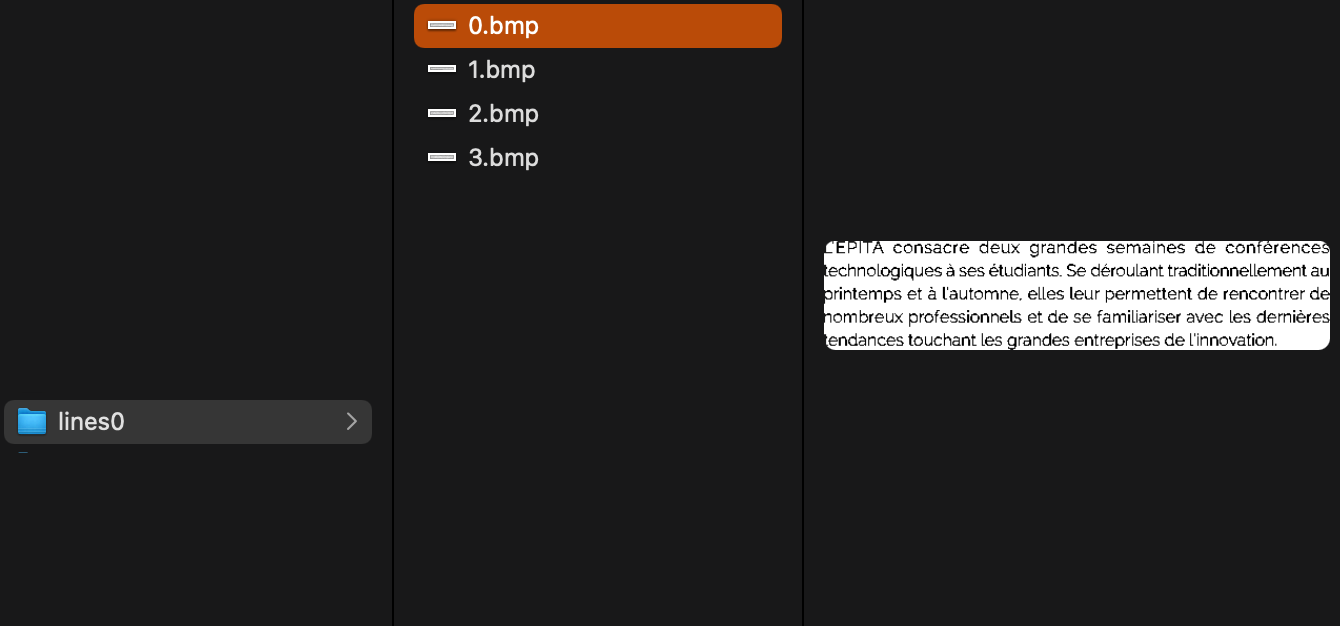
\includegraphics[scale=0.4]{cutColumns}
	\end{center}
	
	\paragraph{}
	Les paragraphes sont parfaitement découpés et prêts à être traités par la suite du programme jusqu'à pouvoir arriver à détecter des caractères.
	
	\subsubsection{Découpage des lignes}
	\paragraph{}
	Le découpage des mots est l'étape suivante que nous avons créée. En effet, les paragraphes sont des blocs de lignes qu'il faut séparer.
	\par Cette partie ressemble très fortement, pour ne pas dire exactement, à la partie précédente. La seule différence apportée se situe au niveau de la tolérance de hauteur entre deux lignes. Pour détecter si on a bien affaire à un changement de ligne, il nous faut regarder l'espace entre la fin supposée de la ligne précédente et le début de la nouvelle. Si cet écart est trop faible, alors on ne considère pas la fin de ligne supposée comme une fin de ligne.
	
	\paragraph{}
	C'est justement le degré considération qui change par rapport au découpage des paragraphes. Ici, on considère un changement si l'écart détecter entre le début et la fin des supposées lignes est supérieur à 0.2 fois la hauteur d'une ligne, comparé à la hauteur elle-même pour la détection de paragraphes.
	\par Dans le code, cela revient à changer les conditions des lignes 17 et 39, on remplaçant \textit{lastLineHeight} par \textit{lastLineHeight * 0.2}. Tout comme le découpage des paragraphes, on dessine les lignes séparatrices puis découpe les lignes pour les stocker dans un dossier dédié. Voici le résultat du découpage des lignes par notre programme: \\
	
	\begin{center}
		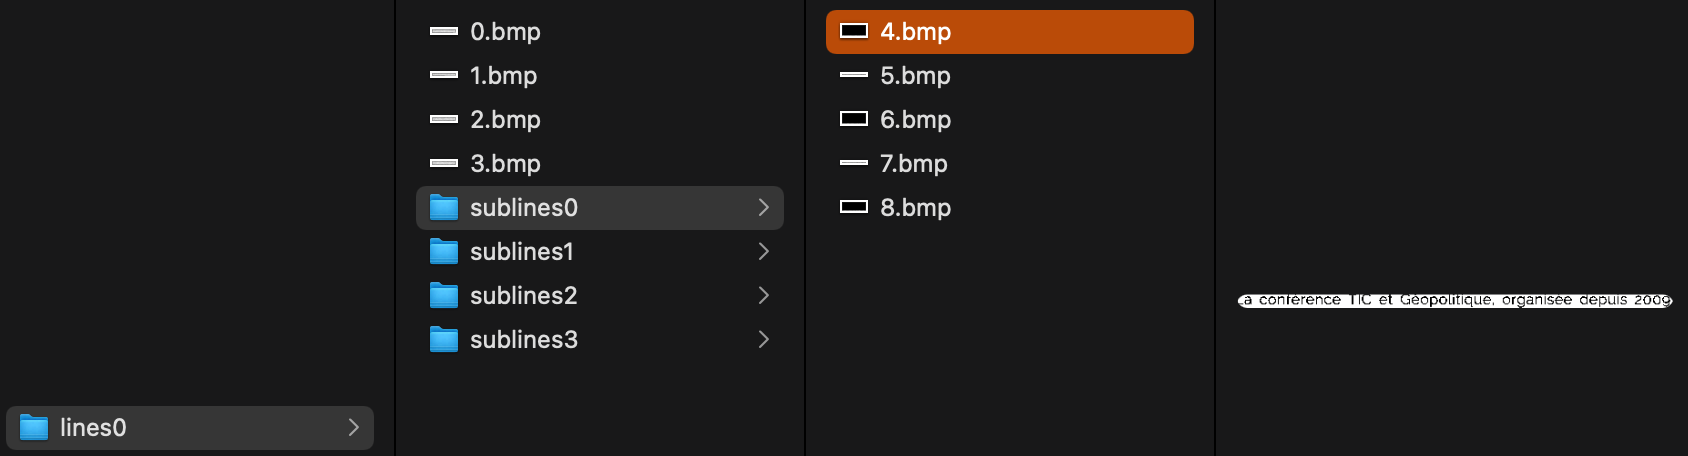
\includegraphics[scale=0.5]{cutLines}
	\end{center}
	
    \subsubsection{Découpage des mots et des caractères}
    \\ 
    \textbf{Première Version:}
	\paragraph{}
	Nous présenter le découpage des mots et des caractères ensemble car ils sont effectués plus ou moins en même temps. En effet, le découpage des caractères reste une étape très délicate à appréhender car elle nécessite de prévoir ou doivent être découpés les caractères.
	
	\paragraph{}
	L'ordre des segmentations voudrait que les mots soient découpés en premiers, puis les caractères ensuite. Au final, c'est plus ou moins ce qui se passe: on dessine les lignes séparant chaque caractère, puis on découpe les mots de la même façon que l'on découpe les colonnes, et enfin on découpe les caractères en utilisant les lignes dessinées auparavant, pour chacun des mots.
	
	\paragraph{}
	Pourquoi faisons nous ces deux découpages en même temps? Tout simplement pour une question de précision sur le découpage des caractères. En effet, notre découpage des caractères se fait en fonction de la largeur moyenne d'un caractère de la phrase en cours de découpage.
	\par Pour être encore plus clair, voici ce qu'il se passe précisément. Nous définissons la largeur moyenne d'un caractère comme \textit{0.5 * (image -> h)}, soit la moitié de la hauteur de l'image (résultat basé sur une comparaison des largeurs moyennes de caractères pour plusieurs polices, celles-ci étant centrées autour de cette valeur). Ensuite, nous parcourons l'image de gauche à droite, c'est-à-dire que nous cherchons le début d'un caractère (tous les pixels ne sont pas blancs sur la hauteur de l'image), puis nous cherchons sa fin (tous les pixels sont blancs). Cette fin n'est pas forcément la bonne, car deux caractères peuvent se chevaucher.
	\par C'est alors qu'intervient notre variable de largeur moyenne d'un caractère. On regarde quelle largeur fait le supposé caractère sélectionné. S'il est x fois plus large que la moyenne, alors nous considérons que x caractères se chevauchent, et on coupe le bloc en x caractères différents. La moyenne est alors modifiée en fonction de la taille des caractères découpés.
	\par Voici pourquoi nous faisons le découpage des caractères avant celui des mots, car plus la phrase contient de caractères, plus on peut être précis sur la façon de les découper.
	
	\paragraph{}
	Voici à quoi ressemble le programme pour le découpage des caractères pour la première version:
	\begin{lstlisting}
	for (int j = 0; j < img -> w; j++)
    {
        fullWhite = fullWhiteHeight(img, j);
        if (!fullWhite && firstCut)
        {
            beginingCharPixel = j;

            /* Draw line for cut (first version usage) */

            firstCut = 0;
        }
        
        if(fullWhite && !firstCut) 
        {
            endingCharPixel = j-1;
            int actualCharLength = abs(endingCharPixel - beginingCharPixel);
            firstCut = 1;
            
            /* Draw line for cut */

            // Bloc is too long
            if (actualCharLength > 2*averageCharLength)
            {
                int times = round(actualCharLength/actualCharLength);
                int middle = actualCharLength/2 + beginingCharPixel;
                for (char k = 1; k <= times; k++){
                    
                    /* Draw line at beginingCharPixel + k*actualCharLength/times for cut */

                }
                nbChars += times;
                averageCharLength = (averageCharLength*(nbChars-times) + actualCharLength)/nbChars;
            }
            else {
                nbChars += 1;
                averageCharLength = (averageCharLength*(nbChars-1) + actualCharLength)/nbChars;
            }
        }
    }
	\end{lstlisting}
	
	\paragraph{}
    L'utilisation du dessin sur l'image de ligne de couleurs n'était au final pas le solution la plus précise, car il était possible que des lignes empiètent sur des pixels importants pour pouvoir reconnaître des caractères ensuite. Nous avons donc établit une autre version plus précise de la segmentation des caractères.\\
    
    
    \textbf{Version finale:}
    \paragraph{}
    Nous avons réfléchit à une solution permettant de stocker facilement les informations de début et de fin des caractères dans l'image, afin de pouvoir les réutiliser dans d'autres fonctions par la suite. La solution retenue à été d'avoir un tableau de positions des indices de début et de fin pour chaque caractères. Ainsi, lorsque le début d'un caractère est détecté, sa position est enregistrée dans un tableau, de même pour la fin d'une détection. Ainsi, le problème de perte de précision n'en n'est plus un.
	
	\paragraph{}
	La même technique est utilisée pour découper colonnes et mots, on regarde quelle taille fait l'espace entre la supposée fin d'un mot et le début de l'autre. Après avoir fait des recherches, un espace représente environ 25\% de la hauteur des caractères. On utilise ainsi cette donnée pour vérifié si l'espace trouvé est supérieur à 22\% de la hauteur de l'image. Cet algorithme fonctionne très bien est découpe brillamment les mots. En voici un exemple: \\
	
	\begin{center}
		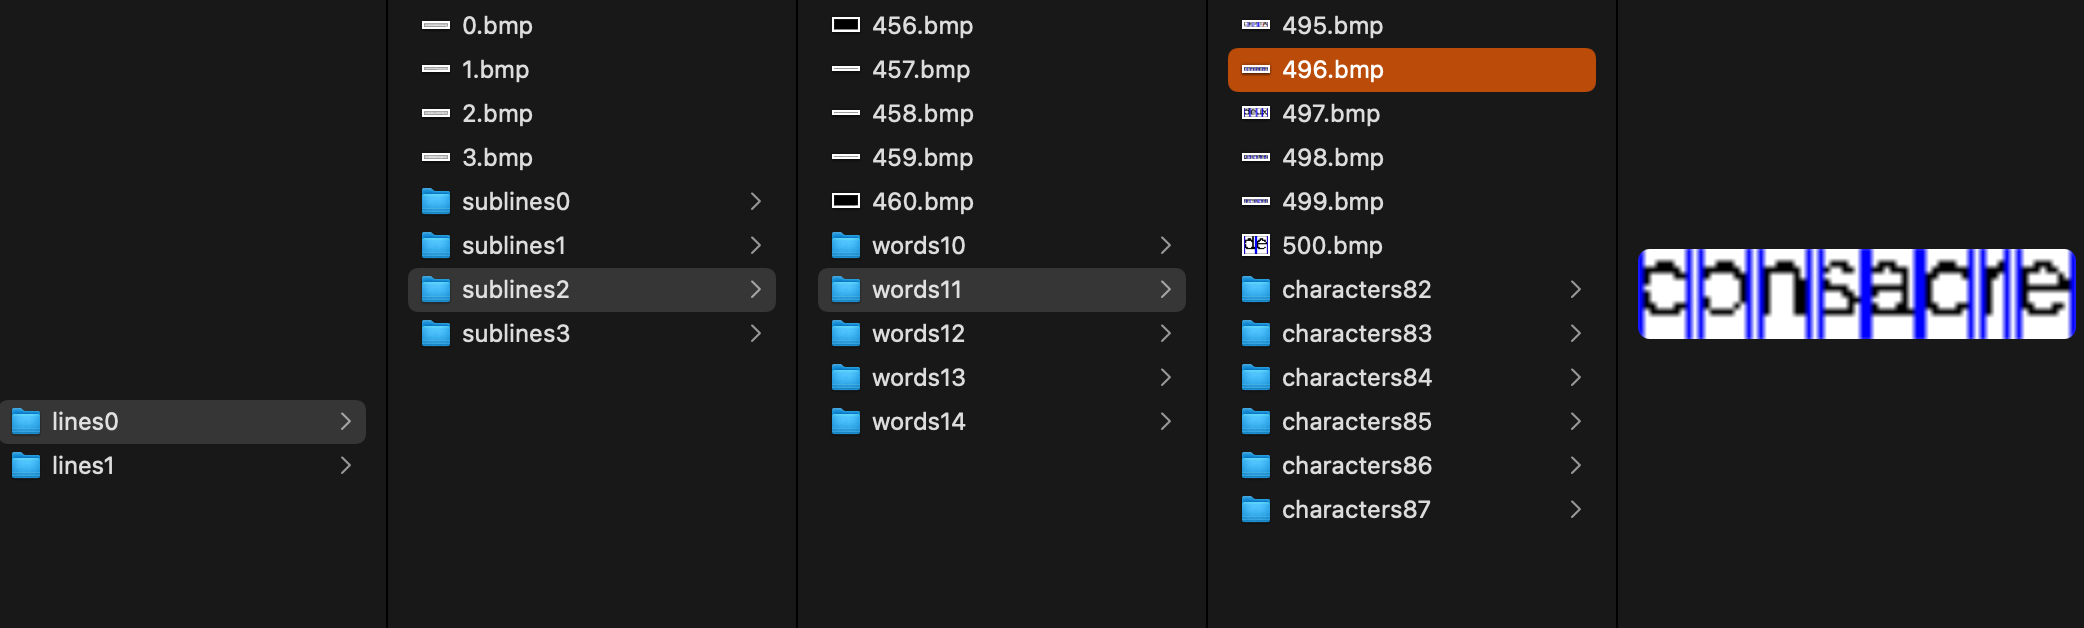
\includegraphics[scale=0.4]{cutWords}
	\end{center}
	
	\paragraph{}Dans ce même dossier se trouvent des dossiers pour les caractères de chaque mots contenus qui contiennent les images en 32x32 pixels avec le caractère positionné en haut à gauche de l'image. Voici donc l'architecture finale de notre projet:
	
	\begin{center}
		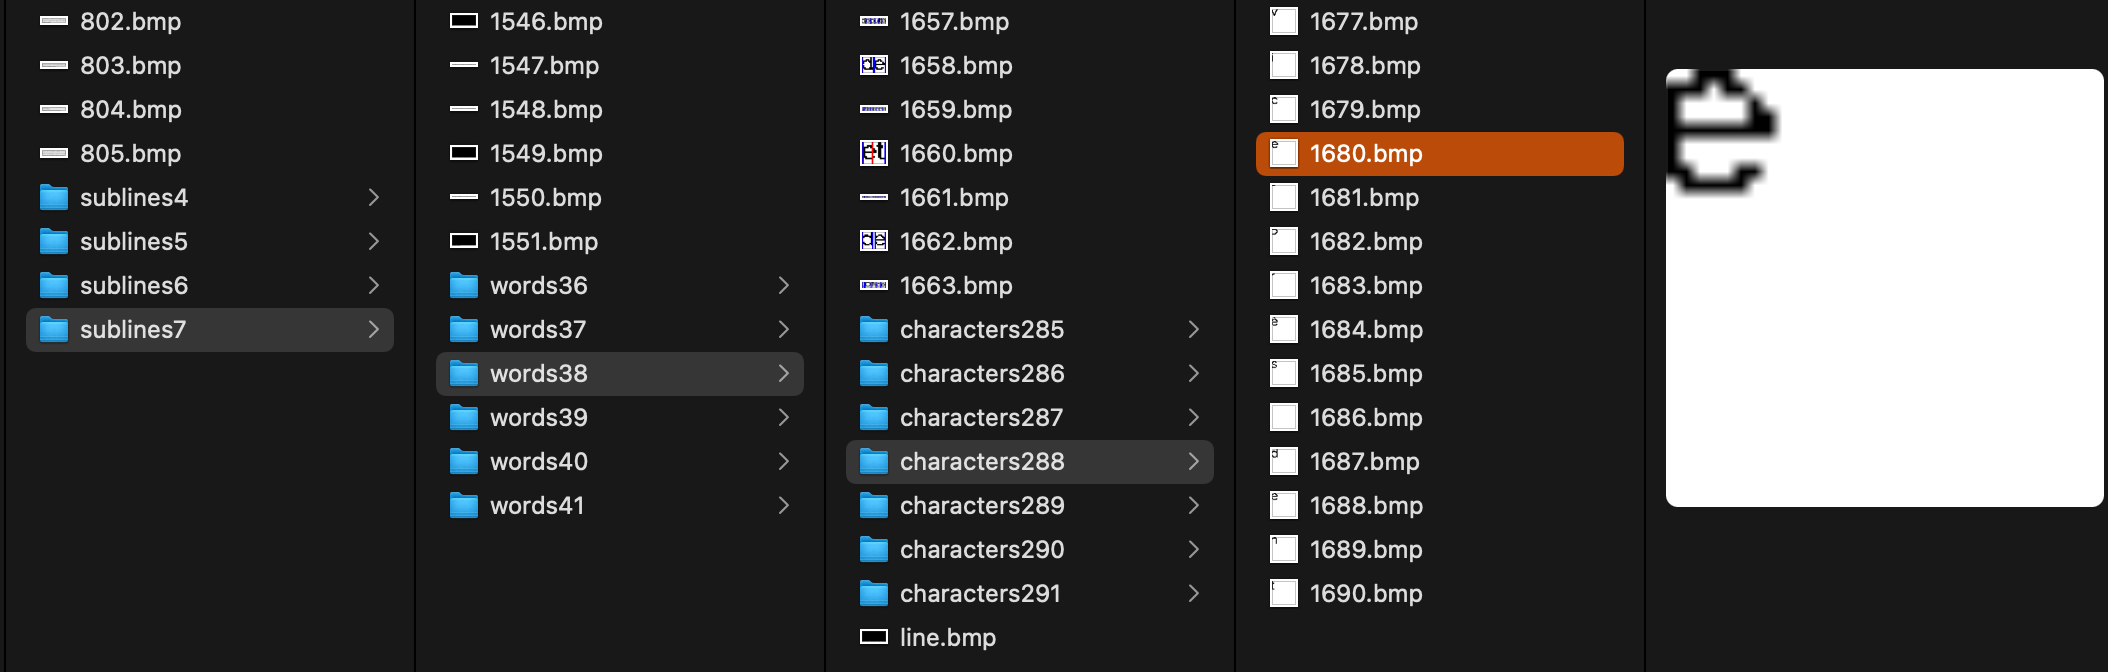
\includegraphics[scale=0.35]{cutCharacters}
	\end{center}
	
    \paragraph{}Cette architecture était une première version pour ce projet, mais nous avons finalement modifier cette dernière, notamment après avoir modifier notre segmentation des caractères pour quelque chose de plus précis. Nous avons au final très peu d'image qui sont sauvegardées après l'exécution du projet, seulement les colonnes et les paragraphes et quelques images d'analyse. \\
    \par Cependant, nous sauvegardons temporairement les images telles que les lignes, les mots et les caractères découpés. En effet, lorsque le projet s'exécute, des dossiers temporaires sont créés et contiennent quelques informations utiles à certaines fonctions, notamment pour récupérer les caractères à envoyer au réseau de neurones. Ces dossiers sont supprimés une fois la compilation terminée.
    
    \subsubsection{Gestion du texte en italique}
    \paragraph{}
    Nous avons constaté que la gestion d'un texte en italique était plus complexe et demandait une approche différente que celle d'un texte classique. Nous avons donc réfléchit à quelles étaient les meilleures options pour pouvoir découper les caractères même s'ils sont en italique.

    \paragraph{}
    Nous nous sommes tout de suite concentrés sur le fait de ne pas dessiner sur l'image pour ensuite découper les caractères à l'aide de ces marques, comme nous avions pu le faire pour les autres types de segmentation. Nous avons donc repris le système de pointeurs, implémenté pour la segmentation classique, qui stocke le début et la fin d'un caractère dans une tableau, nous permettant ensuite de découper et enregistrer le caractère dans une nouvelle petite image. Cette nouvelle image sera ensuite envoyée dans le réseau de neurones pour reconnaître le caractère écrit.

    \paragraph{}
    Pour ce qui est de détecter le début et la fin d'un caractère en italique, nous avons tout simplement repris le système codé pour une écriture classique et nous avons fait en sorte qu'il soit incliné. C'est-à-dire que nous vérifions que l'image est toute blanche en hauteur sur un pixel défini, tout ceci en fonction de ce qui est recherché (début ou fin de caractère). Nous ne testons cependant plus vraiment si l'image est toute blanche en hauteur, mais plutôt si elle est toute blanche suivant un angle d'inclinaison donné, qui correspond à l'angle d'inclinaison d'un texte en italique classique. Voici l'algorithme: \\

    \begin{lstlisting}
        if (!fullWhite && firstCut)
        {
            // Saving beginning index 
            // (exclusive position: where we will need to cut)
            allPositions[currentIndex] = j - 1;
            currentIndex ++;

            // Drawing lines for test
            int put_j = j != 0 ? j - 1 : 0; 
            beginingCharPixel = j;
            int jj = j;
            for (int i = 0; i < img -> h && jj > -1; i++)
            {
                pixel = SDL_MapRGB(img_copy -> format, 0, 0, 255);
                putpixel(img_copy, jj, i, pixel);

                // Updating indexes for italic segmentation (mod = 5)
                if (i % mod == mod-1){
                    jj--;
                }
            }
            firstCut = 0;
        }
        
        if(fullWhite && !firstCut) 
        {
            // Saving ending index
            // (exclusive position: where we will need to cut)
            allPositions[currentIndex] = j + 1;

            // Drawing lines for test
            endingCharPixel = j - 1;
            int actualCharLength = abs(endingCharPixel - beginingCharPixel + 1);
            int jj = j;
            for (int i = 0; i < img -> h && jj > -1; i++)
            {
                pixel = SDL_MapRGB(img_copy -> format, 0, 0, 255);
                putpixel(img_copy, jj, i, pixel);

                // Updating indexes for italic segmentation (mod = 5)
                if (i % mod == mod-1){
                    jj--;
                }
            }
            firstCut = 1;
        }
    \end{lstlisting}

    \paragraph{}
    On remarque que cet extrait de code gère le cas où ledébut d'un caractère est trouvé (première boucle), ainsi que le cas où la fin d'un caractère est trouvée (deuxième boucle). Leur fonctionnement est plutôt similaire et nous allons décortiquer la première boucle.
    \par Tout d'abord, on sauvegarde la position du caractère dans notre tableau 'allPositions' qui les stocke. Ensuite, on dessine sur l'image pour voir comment la segmentation s'est déroulée. Dessiner sur l'image est juste un indicateur pour voir comment le programme fonctionne et permet de comprendre comment on détecte que l'image est toute blanche sur la partie souhaitée. La façon dont se passe la detection inclinée est la suivante: on fait une boucle sur toute la hauteur de l'image, puis tous les 5 itérations, on décale le pixel de recherche de 1 vers la gauche, ce qui permet au final d'avoir une détection en biais. Voici le résulat d'une segmentation sur un texte en italique: \\

    $IMAGE_CARACTERES_ITALIQUE$

    \paragraph{}
    Nous avons également appliqué se processus de détection inclinée pour la segmentation des mots. L'exact même algorithme est appliqué, et il permet d'être plus précis sur la détection des mots. Voici le résultat obtenu:

    $IMAGE_MOTS_ITALIQUE$
	
\newpage

\rhead{\textit{Réseau de neurones}\vspace{0.25cm}}
\section{Réseau de neurones}

\subsection{Avancées}

\subsubsection{Fonction XOR}

\paragraph{} La première étape pour obtenir un bon réseau de neurones était de développer un réseau capable d'apprendre la fonction XOR. Cela a pour avantage que le réseau serait rapide à entraîner, le réseau n'a que 2 entrées pour une seule sortie, et seulement 4 motifs d'entraînements.

\begin{center}
\vspace*{0.2cm}
\begin{tabular}{|l|l|c|r|}
  \hline
  & entrée 1 & entrée 2 & sortie \\
  \hline
  Motif 1 & 0 & 0 & 0 \\
  Motif 2 & 0 & 1 & 1 \\
  Motif 3 & 1 & 0 & 1 \\
  Motif 4 & 1 & 1 & 0 \\
  \hline
\end{tabular}
\end{center}


\paragraph{}N'étant alors pas tout à fait à l'aise avec ce "nouveau" langage qu'est le C, j'ai d'abord cherché à faire ce réseau en Python, un langage que je maîtrise depuis plusieurs années. J'ai donc cherché de l'aide et des exemples de réseaux de neurones par rétropropagation en Python, mais la plupart des résultats utilisaient le module Numpy pour la manipulation de matrice ainsi que certains calculs, or, en C, tout cela doit être traité manuellement.

\paragraph{}Après plusieurs heures de recherche, je suis tombé sur un très bon tutoriel qui expliquait en détail le fonctionnement d'un tel programme, avec des exemples en C++. J'ai facilement réussi à refaire le programme en Python, puis en C.

\paragraph{}Ensuite, pour voir si un tel réseau était adaptable à d'autres algorithmes, j'ai essayé de lui faire apprendre d'autres motifs, comme une fonction qui à partir de trois entrées, renvoie 1 si au moins 2 sont à 1 (et 0 sinon).

\subsubsection{Reconnaissance de caractères}

\paragraph{}Une seconde étape était de prévoir une structure pour notre réseau de neurones.
Au final, le réseau qui apprendra à reconnaître des caractères est un réseau semblable à notre réseau XOR, avec un nombre d'entrées égal à nombre de pixel dans une image, et le nombre de sorties serait égal au nombre de caractères à reconnaître.

\paragraph{}Les entrées sont des doubles compris entre 0 et 1, un 0 correspond à un pixel dont la couleur est celle du fond de l'image, un 1 correspond à un pixel de la couleur d'écriture du caractère.

\paragraph{}Les images qui lui seront transmises auront une taille de 32$\times$32 et seront collées au coin supérieur gauche. Le réseau a donc 1024 entrées.

\paragraph{}Le nombre de sorties est égal au nombre de caractères à reconnaître. On suppose donc que la sortie ayant la plus grande valeur correspond au caractère reconnu.

\paragraph{} Dès la réception du cahier des charges le 10 septembre, j'ai écris un programme C qui à l'aide de SDL2, lit des images et enregistre la valeur des pixels dans un tableau. Ce programme est encore utilisé aujourd'hui, mais sera surement modifié d'ici à la fin du projet pour mieux correspondre avec le traitement de l'image effectué par mes camarades.

\paragraph{}Ensuite, il nous fallait un catalogue d'images (dataset) qui pourrait être utilisé pour l'entraînement et les tests du réseau. Les catalogues trouvés sur internet étaient très limités (taille des images ne correspondant pas, trop peu d'images,…), la meilleure solution était de créer nos propres datasets.

\paragraph{}Pour cela, j'ai écris un petit script en Python qui génère des images avec un caractère dessus (grâce à la bibliothèque PIL). La police, couleur et taille sont aléatoires afin d'obtenir un entraînement plus diversifié.

\paragraph{}Le premier réseau devait apprendre à reconnaître les caractères numériques 0 à 9. Les résultats n'étaient au début pas très probants. Et pour cause: les poids et biais des neurones étaient mal initialisés (Ils étaient initialisés entre 0 et 1 au lieu de entre -0.5 et 0.5). Une fois ce problème corrigé, le réseau arrivait à apprendre et reconnaissait les caractères avec une précision de 67\% environ. Deux problèmes se posaient alors:

\begin{itemize}
	\item Le réseau ne montait pas au dessus de 67\% de réussite
	\item Il avait besoin de beaucoup de neurones (plus de 1000) dans sa couche intermédiaire.
\end{itemize}

\paragraph{} Ces problèmes m'ont pas mal pris la tête, et m'ont obligé à revoir l'ensemble du programme.
Au bout de deux semaines de migraines, l'origine du problème m'est apparue: la dérivée de la fonction Sigmoïde était mal implémentée.

La dérivée de la sigmoïde s'écrit comme ceci:

\begin{center}
	$\frac{d\sigma(x)}{dx} = \sigma(x)\dot{}(1 - \sigma(x))$
\end{center}

\paragraph{}Or, les paramètres récupérés et qui passent dans cette fonction sont déjà $\sigma(x)$. Du coup, la dérivée était au final calculée comme $\sigma^2(x)\dot{}(1 - \sigma^2(x))$

\paragraph{}Une fois ce problème résolu, on a obtenu des résultats proches de 95\% pour une couche intermédiaire de seulement 760 neurones.

\subsection{Fonctionnement}

\subsubsection{Scripting}

\paragraph{}Une fois que j'étais sûr que le réseau était bien en train d'apprendre, je me suis chargé du scripting, c'est à dire de créer des structs et des fonctions qui permettent d'interagir avec le réseau plutôt que de tout avoir dans un même fichier .c.

Le réseau de neurones tourne donc autour de deux structs: 

\begin{itemize}
	\item MMImage est une struct qui contient toutes les informations caractérisant une image pour une prédiction (dimensions de l'image, valeurs des pixels, …) ou le training (caractère que c'est vraiment, …)
	\item MMNetwork, qui contient les informations à propos d'un réseau de neurones (nombre d'entrées, sorties, neurones, les poids et les biais)
\end{itemize}

\paragraph{}J'ai implémenté des fonctions autour de ces structs, comme la fonction LoadDataset, qui permet de charger un dataset complet en mémoire, ou LoadImage qui permet de ne charger qu'une seule image.

\begin{lstlisting}
MMImage*		LoadDataset(int noChars, int imagesPerChar);
MMImage		LoadImage(char* path);
\end{lstlisting}

\paragraph{}Concernant MMNetwork, on peut initialiser un réseau grâce à la fonction InitNetwork.
Pour libérer la mémoire, on a la fonction DestroyNetwork.

\begin{lstlisting}
MMNetwork InitNetwork(unsigned int numInputs, unsigned short numHiddenNodes, unsigned int numOutputs);
void DestroyNetwork(struct MMNetwork n);

\end{lstlisting}

\paragraph{}L'avantage de MMNetwork, c'est qu'il peut être enregistré et chargé dans des fichiers. Cela sert notamment à sauvegarder l'état d'un réseau entraîné pour pouvoir le récupérer par la suite pour faire des prédictions.

\begin{lstlisting}
void SaveNetwork(MMNetwork n, char* path);
MMNetwork LoadNetwork(char* path);
\end{lstlisting}


\paragraph{}
À partir de là, les bases sont posées pour effectuer n'importe quel type d'opérations avec les réseaux. En effet, une simple prédiction peut se faire avec la fonction Predict, qui à partir d'un MMImage et d'un MMNetwork, renvoie les valeurs de la couche de sortie du réseau, qui peut être analysée par la fonction OutputChar.

\begin{lstlisting}
double*	Predict(MMNetwork network, const MMImage* image);
char OutputChar(double* outputLayer);
\end{lstlisting}

\textbf{Exemple de programme:}

\paragraph{}Analysons maintenant le programme suivant, qui permet de prédire le caractère présent sur une image:


\begin{lstlisting}
#include <stdio.h>
#include "LambdaNeuralNetwork.h"

int main(int argc, const char* argv[]) {

	MMImage img = LoadImage("/Users/maxime/Documents/OCR/W.bmp");
	MMNetwork n = LoadNetwork("/Users/maxime/Documents/OCR/IA");
	
	double* output = Predict(n, &img);
	char character = OutputChar(output);
	
	printf("Recognized as a %d\n", character);
	printf("\n");
	
	return 0;
}
\end{lstlisting}


\begin{itemize}
	\item Ligne 2: On inclut le header principal, qui définit toutes les fonctions et structs utilisées pour la prédiction et l'utilisation des réseaux de neurones du projet.
	\item Ligne 6: On charge une image à partir de son chemin d'accès dans une variable img
	\item Ligne 7: On charge le réseau précédemment entraîné à partir du chemin où il a été enregistré dans une variable n
	\item Ligne 9: On fait une prédiction sur l'image img par le réseau n. Les valeurs de la couche de sortie sont enregistrées dans une variable output.
	\item Ligne 10: À partir de la couche de sortie output, on récupère le caractère correspondant. C'est ce caractère qui est écrit sur l'image.
\end{itemize}

\paragraph{}Juste ces 4 lignes permettent de faire une prédiction sur le caractère écrit sur une image.

\newpage

\subsubsection{Compilation}
Le réseau de neurones a été entièrement programmé sur l'IDE Xcode, et a été organisé en 3 projets:


\begin{itemize}
	\item La library "LambdaNeuralNetwork" qui contient les fonctions et les structs
	\item Un programme "Learning" qui s'occupe de l'entraînement du réseau
	\item Un programme "Analyze" qui va effectuer des prédiction sur un testing-set afin d'obtenir un taux de réussite sur un réseau après entraînement
\end{itemize}
Un Makefile permet de compiler chacun de ces projets:

\begin{lstlisting}
make lib
make analyze
make learning

make all
make clean
\end{lstlisting}

Effectuer un make pour compiler un des programme va créer l'exécutable correspondant dans un dossier bin.
Compiler la lib va créer un dossier lib contenant des fichiers .o. Le fichier principal LambdaNeuralNetwork.o est le lien vers tous les autres .o.

Importer le fichier LambdaNeuralNetwork.o et include le fichier "include/LambdaNeuralNetwork.h" suffit pour pouvoir utiliser toutes les fonction et les structs.


\subsubsection{Fonctionnement du réseau}

\paragraph{}L'apprentissage du réseau utilise un algorithme du gardient stochastique (Stochastic Gradient Descent), une "variante" de la descente du gradient qui a pour particularité de l'utiliser qu'un seul élément (en l'occurrence une image) choisi aléatoirement du training-set à la fois pour modifier les poids. (Un algorithme standard de descente du gradient utilisera tous les éléments en même temps).

\paragraph{}Voici un schéma simplifié de notre réseau.
(Le réseau comporte 1024 entrées, 760 neurones cachés, et 78 sorties. Pour des raisons de clarté, je n'ai représenté que certains d'entre eux.)

\begin{center}
	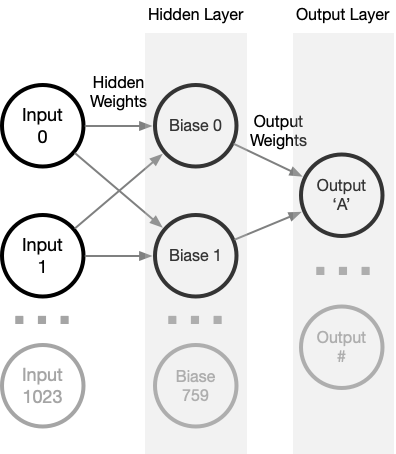
\includegraphics[scale=0.5]{Neuron}
\end{center}

\paragraph{} Chaque entrée influera sur chaque neurone caché par l’intermédiaire d’un poids caché (hidden weight) et du biais du neurone caché.
De même, chaque neurone caché influera sur chaque neurone de sortie par l’intermédiaire d’un poids de sortie (output weight) et du biais du neurone de sortie.
À chaque itération de l’apprentissage, une valeur est calculée pour chaque neurone caché:
\newline

$hiddenLayer_j=\sigma(hiddenLayerBias_j+\sum_i input_i\times hiddenWeight_{i\rightarrow j})$

(où $hiddenLayerBias_j$ est le biais du neurone, $hiddenWeight_{i\rightarrow j}$ le poids de la transition de l’entrée i vers le neurone)

\vspace*{0.3cm}

\paragraph{} Idem pour les valeurs de la couche de sortie:\newline

$outputLayer_k=\sigma(outputLayerBias_k+\sum_i hiddenLayer_j\times outputWeight_{j\rightarrow k})$


(où $outputLayerBias_k$ est le biais du neurone, $outputWeight_{j\rightarrow k}$ le poids de la transition du neurone caché i vers le neurone de sortie)

\begin{center}
	
\includegraphics[scale=0.5]{Meme}
\end{center}

\newpage
\rhead{\textit{Correcteur orthographique}\vspace{0.25cm}}
\section{Correcteur orthographique}

\subsection{L'objectif}

\paragraph{}Notre but ici était de pouvoir corriger les fautes dans un texte scanné par l’OCR et avoir une vérification supplémentaire de ce qu’a renvoyé le réseau de neurones.

\subsection{La ponctuation}

\paragraph{}
Pour vérifier la ponctuation d’un texte nous avons opté pour un ensemble de fonction vérifiant chacune des règles particulières de la ponctuation de la langue française. Par exemple, le code ci-dessous vérifie s'il y a bien un espace après le point et une majuscule.

\paragraph{}Il existe deux fonctions similaires respectivement pour les règles du point d’interrogation et celui d’exclamation. Ces fonctions ont pour vocation d'être utilisé avec une main qui leur enverrait l’index des points dans un texte.

\subsection{La cohérence}
\paragraph{}Cette fonction a vu le jour pour palier un problème du réseau de neurones. En effet, il pouvait arriver que l'IA confonde une majuscule avec une minuscule. La fonction ci-dessous vérifie alors s’il y a plus de lettre majuscule ou minuscule dans le mot et change le tout.  Cette fonction nous apporte une sécurité supplémentaire.

\subsection{La distance de Levensthein}
\paragraph{}Pour concevoir un correcteur orthographique assez rapide pour être utilisé, nous avons dû faire de nombreuses recherches qui nous ont conduit vers la matrice de Levenshtein. Cette dernière est la méthode de calcul la plus rapide que nous avons pu implémenter et elle compare n’importe quel mot avec tous les autres du dictionnaire français (336 524 mots au total) en 0.5 seconde. A l'heure actuelle, le correcteur orthographique est utilisable pour corriger 1 mot à la fois. Cependant, le temps actuel bien que déjà très bon n’est pas suffisamment faible pour pouvoir être utilisé à une plus grande échelle. Nous avons donc pour objectif pour la prochaine soutenance d’améliorer ce temps notamment par l’utilisation d’une table de hachage ou bien par la comparaison de triplet de caractères et pour pouvoir améliorer nos chances de réussite de correction d’un mot dans le même temps. La plus grande difficulté pour nous aura été de trouver un moyen de contourner l'utilisation d'une IA et d’apporter des solutions de correction viable sans l’utilisation des habitudes de l’utilisateur.


\newpage
\rhead{\textit{Command parser}\vspace{0.25cm}}
\section{Command parser}

\subsection{L'objectif}

\paragraph{}Notre but ici était de permettre l'utilisation de notre programme via des lignes de commandes dans un premier temps avant de réaliser l'interface graphique.

\paragraph{}Nous avons donc ajouté 3 commandes qui permettent d'exécuter des fonctionnalités clés telles que nos filtres, notre niveau de gris ainsi que la segmentation d'une image quelconque.

\subsection{Grayscale}

\paragraph{}C'est une fonction qui a besoin de 2 paramètres, le premier est le chemin de l'image d'origine et le deuxième le chemin auquel l'image en niveau de gris sera sauvegardée. Si les deux paramètres ne sont pas entrés ou bien que l'image entrée en paramètre ne peut être chargée, le programme s'arrête et renvoie un message d'erreur.

\begin{lstlisting}

	if (argc == 4) {
		SDL_Surface *imgDefault;
		imgDefault = SDL_LoadBMP(argv[2]);
		if (!imgDefault) {
			printf("Error: unable to find bmp file at %s\n", argv[2]);
			return 1;
		}
		imgDefault = grayscale(imgDefault, 1, argv[3]);
		return 0;
	}
	else {
		printf("Lambda: Grayscale take exactly 2 parameters but was called with %i parameter(s)\n", argc - 2);
		return 1;
	}
\end{lstlisting}

\paragraph{}Ici, l'objectif est de couvrir tous les cas d'utilisation et d'éviter les crash de notre programme. Ainsi la fonction n'est appelée uniquement lorsque tous les paramètres sont entrés et la fonction grayscale renvoi un booléen indiquant qu'une erreur s'est produite pendant l'exécution et ainsi permet au parser de prévenir l'utilisateur.

\subsection{Filtres}

\paragraph{}Il fallait ajouter la possibilité d'utiliser les filtres de notre programme. Pour cela, nous avons créé la fonction filters à notre programme. Celle ci applique une augmentation des contrastes de façon systématique et la reduction de bruits si le 3ème paramètre est vrai.

\paragraph{}De la même façon que les autres commandes, il ne faut pas faire crasher le programme de façon involontaire. C'est pour cela que nous avons fait en sorte de sortir des exceptions et d'arrêter le programme dès qu'une erreur peut se produire. Voici le code pour cette commande:

\begin{lstlisting}
	if (argc == 4 || argc == 5) {
			SDL_Surface *imgDefault;
			imgDefault = SDL_LoadBMP(argv[2]);
			if (!imgDefault) {
				printf("Error: unable to find bmp file at %s\n", argv[2]);
				return 1;
			}
			if (argc == 5 && strcmp(argv[4], "true") == 0)
			{
				imgDefault = contrast(imgDefault);
				printf("Lambda: Noise reduction ended successfully\n");
			}
			
			imgDefault = contrast(imgDefault);
			printf("Lambda: Contrast ended successfully\n");
			SDL_SaveBMP(imgDefault, argv[3]);
			return 0;
		}
		else {
			printf("Lambda: Filters take 1 or 2 paramaters but was called with %i parameter(s)\n", argc - 2);
			return 1;
		}
\end{lstlisting}

\subsection{Segmentation}

\subsubsection{Segmentation complète}
La fonction de segmentation s'exécute avec simplement un paramètre: le chemin de l'image qu'il faut segmenter. Pour le reste, tout est géré via une architecture de dossiers et fichiers précise, l'utilisateur n'a pour l'instant pas le choix de ce dernier.

\begin{lstlisting}
	if (argc == 3) {
		if (!fullSegmentation(argv[2])) {
			printf("Lambda: Error during segmentation execution\n");
			return 1;
		}
		printf("Lambda: Segmentation ended successfully\n");
		return 0;
	}
	else {
		printf("Lambda: Segmentation take exactly 1 paramater but was called with %i parameter(s)\n", argc - 2);
		return 1;
	}
\end{lstlisting}

\subsubsection{Segmentation d'une ligne}

\paragraph{}Notre programme gérant le multi-colonnes, nous avons dans l'idée d'ajouter une option pour que l'utilisateur indique si oui ou non l'image entrée est sur une colonne ou sur plusieurs. Voici la fonction qui gère ce cas:

\begin{lstlisting}
	if (argc == 3) {
			SDL_Surface *img;
			img = SDL_LoadBMP(argv[2]);
			img = cutCharacters(img, "exampleChars/");
			if (!img) {
				printf("Lambda: Error during segmentation execution\n");
				return 1;
			}
			removeLinesForCharacters(img, "chars/");
			printf("Lambda: Segmentation ended successfully\n");
			return 0;
		}
		else {
			printf("Lambda: Characters take exactly 1 paramater but was called with %i parameter(s)\n", argc - 2);
			return 1;
		}
\end{lstlisting}

\newpage
\rhead{\textit{Avancement}\vspace{0.25cm}}
\section{Notre avancement et répartition des tâches}


\subsection{Répartition des tâches à la première soutenance}

\paragraph{} Nous vous avons présenté les fonctionnalités de notre projet sans dire qui était en charge de ces dernières. Ce tableau est le récapitulatif global de nos tâches respectives pour la première soutenance, le X signifie que la personne a participé à cette tâche. L'objectif ici est de clarifier nos rôles, nous formons un seul groupe qui progresse et se donne des objectifs en fonction des possibilités et envies de chacun. Le nombre de tâches réalisées n'a pas de rapport avec l'investissement dans le projet car la complexité est différente.
\begin{center}
\vspace*{0.2cm}
\begin{tabular}{|l|c|c|c|c|}
  \hline
  & Quentin & Maxime & Charles & Nathan \\
  \hline
  Pré-traitement & X &  & X &  \\
  \hline
  Segmentation de l'image & X &  & X &  \\
  \hline
  Réseau de neurones &  & X &  &  \\
  \hline
  Correcteur orthographique &  &  &  & X \\
  \hline
  Command parser &  &  & X &  \\
  \hline
\end{tabular}
\end{center}

\vspace*{1cm}

\subsection{Nos objectifs et envies}

\paragraph{}La deuxième soutenance sera la dernière pour ce projet, il faut donc qu'il soit terminé d'ici là. Nous devons donc mettre tout en oeuvre pour lier la segmentation en caractères de notre image source avec la reconnaissance de ces derniers pour permettre à l'utilisateur de récupérer son texte.

\paragraph{}Il nous faut aussi commencer l'interface graphique pour donner vie à notre projet et lui faire dépasser le stade des lignes de commandes. Nous avons déjà commencé à utiliser pour GTK et Glade pour créer cette dernière et elle sera terminée pour la deuxième soutenance. L'objectif est créer une interface en adéquation avec le style graphique que nous avons mis au point pour le groupe.

\paragraph{}La finalisation du correcteur orthographique est une étape importante pour le projet. Elle ajouterai une fonctionnalité utile pour l'utilisateur. Cela nous apportera beaucoup dans la compréhension de l'implémentation d'un correcteur orthographique et sa réalisation et nous fera réfléchir à l'optimisation de notre programme pour ne pas perdre trop de temps sur la correction. 

\paragraph{}L'IA doit encore être entrainée pour avoir un taux d'erreur le plus bas possible et reconnaître au mieux les caractères de l'image. Il faut penser à la reconnaissance des accents, virgules, points, ...

\paragraph{}Nous devons aussi penser à améliorer notre segmentation des caractères pour éviter les problèmes auxquels nous sommes confrontés aujourd'hui et peut être créer un réseau de neurones qui pourrait apprendre à reconnaître des caractères sur une ligne grâce si nous avons le temps.

\newpage
\subsection{Utilisation du programme}

\paragraph{}Il faut d'abord générer notre exécutable en entrant la commande make dans le dossier parent de notre projet. Le nom de l'exécutable est Lambda il faut donc utiliser ./Lambda pour commencer à utiliser notre programme. Voici la liste des fonctions qui sont utilisables:

\vspace*{0.5cm}

\begin{lstlisting}
	./Lambda grayscale "image_path" "destination"
	// Appliquer le filtre de niveaux de gris sur l'image et l'enregistrer dans la destination
\end{lstlisting}


\begin{lstlisting}
	./Lambda filters "image_path" "destination" true 
	// Applique l'augmentation de contrastes sur l'image et la sauvegarde dans la destination
	// Dernier argument optionnel: permet d'appliquer la reduction de bruits
\end{lstlisting}

\begin{lstlisting}
	./Lambda column "image_path"
	// Applique la segmentation partielle en colonnes de l'image et créer l'architecture resultColumn/*.bmp
\end{lstlisting}

\begin{lstlisting}
	./Lambda paragraph "image_path"
	// Applique la segmentation partielle en paragraphes de l'image et créer l'architecture resultParagraph/*.bmp
\end{lstlisting}

\begin{lstlisting}
	./Lambda line "image_path"
	// Applique la segmentation partielle en lignes de l'image et créer l'architecture resultLine/*.bmp
\end{lstlisting}

\begin{lstlisting}
	./Lambda word "image_path"
	// Applique la segmentation partielle en mots de l'image et créer l'architecture resultWord/*.bmp
\end{lstlisting}

\begin{lstlisting}
	./Lambda characters "image_path"
	// Applique la segmentation partielle et génère l'architecture de dossiers/fichiers
\end{lstlisting}



\newpage
\rhead{\textit{Conclusion}\vspace{0.25cm}}
\section{Conclusion}

\paragraph{}Ce projet est très motivant pour nous tous. Il nous permet d'expérimenter et de réfléchir à des problématiques intéressantes que nous prenons comme des défis. 

\paragraph{}Nous avons fortement aimé le sujet ainsi que le cahier des charges de ce projet, et nous nous sommes ainsi entièrement investis dans sa réalisation. Nous sommes toujours autant motivés par ce projet, malgré les hauts et les bas qui, pour les derniers, peuvent être vraiment complexes à solutionner.\\

\paragraph{}Nous vous avons ici présenté ce que nous avons pu réaliser en un mois dans le respect des consignes proposées par le cahier des charges.


\newpage


\end{document}
